\documentclass[10pt,a4paper]{article}
\usepackage[utf8]{inputenc}
\usepackage{geometry}
\geometry{margin=0.75in}
\usepackage{graphicx}
\usepackage{float}
\usepackage{hyperref}
\usepackage{amsmath}
\usepackage{fancyhdr}



\pagestyle{fancy}
\fancyhf{}
\rhead{\footnotesize Data Storm 7.0 - Team InsightAI}
\lhead{\footnotesize Technical Submission}
\cfoot{\footnotesize Page \thepage \ of 5}

\begin{document}

% --- PAGE 1: COVER PAGE ---
\begin{titlepage}
    \centering
    \vspace*{1in}
    {\Huge \textbf{Data Storm 7.0: Modeling Unconstrained Latent Demand}} \\
    \vspace{0.5in}
    {\Large \textbf{Team InsightAI - Final Technical Report}} \\
    \vspace{1in}
    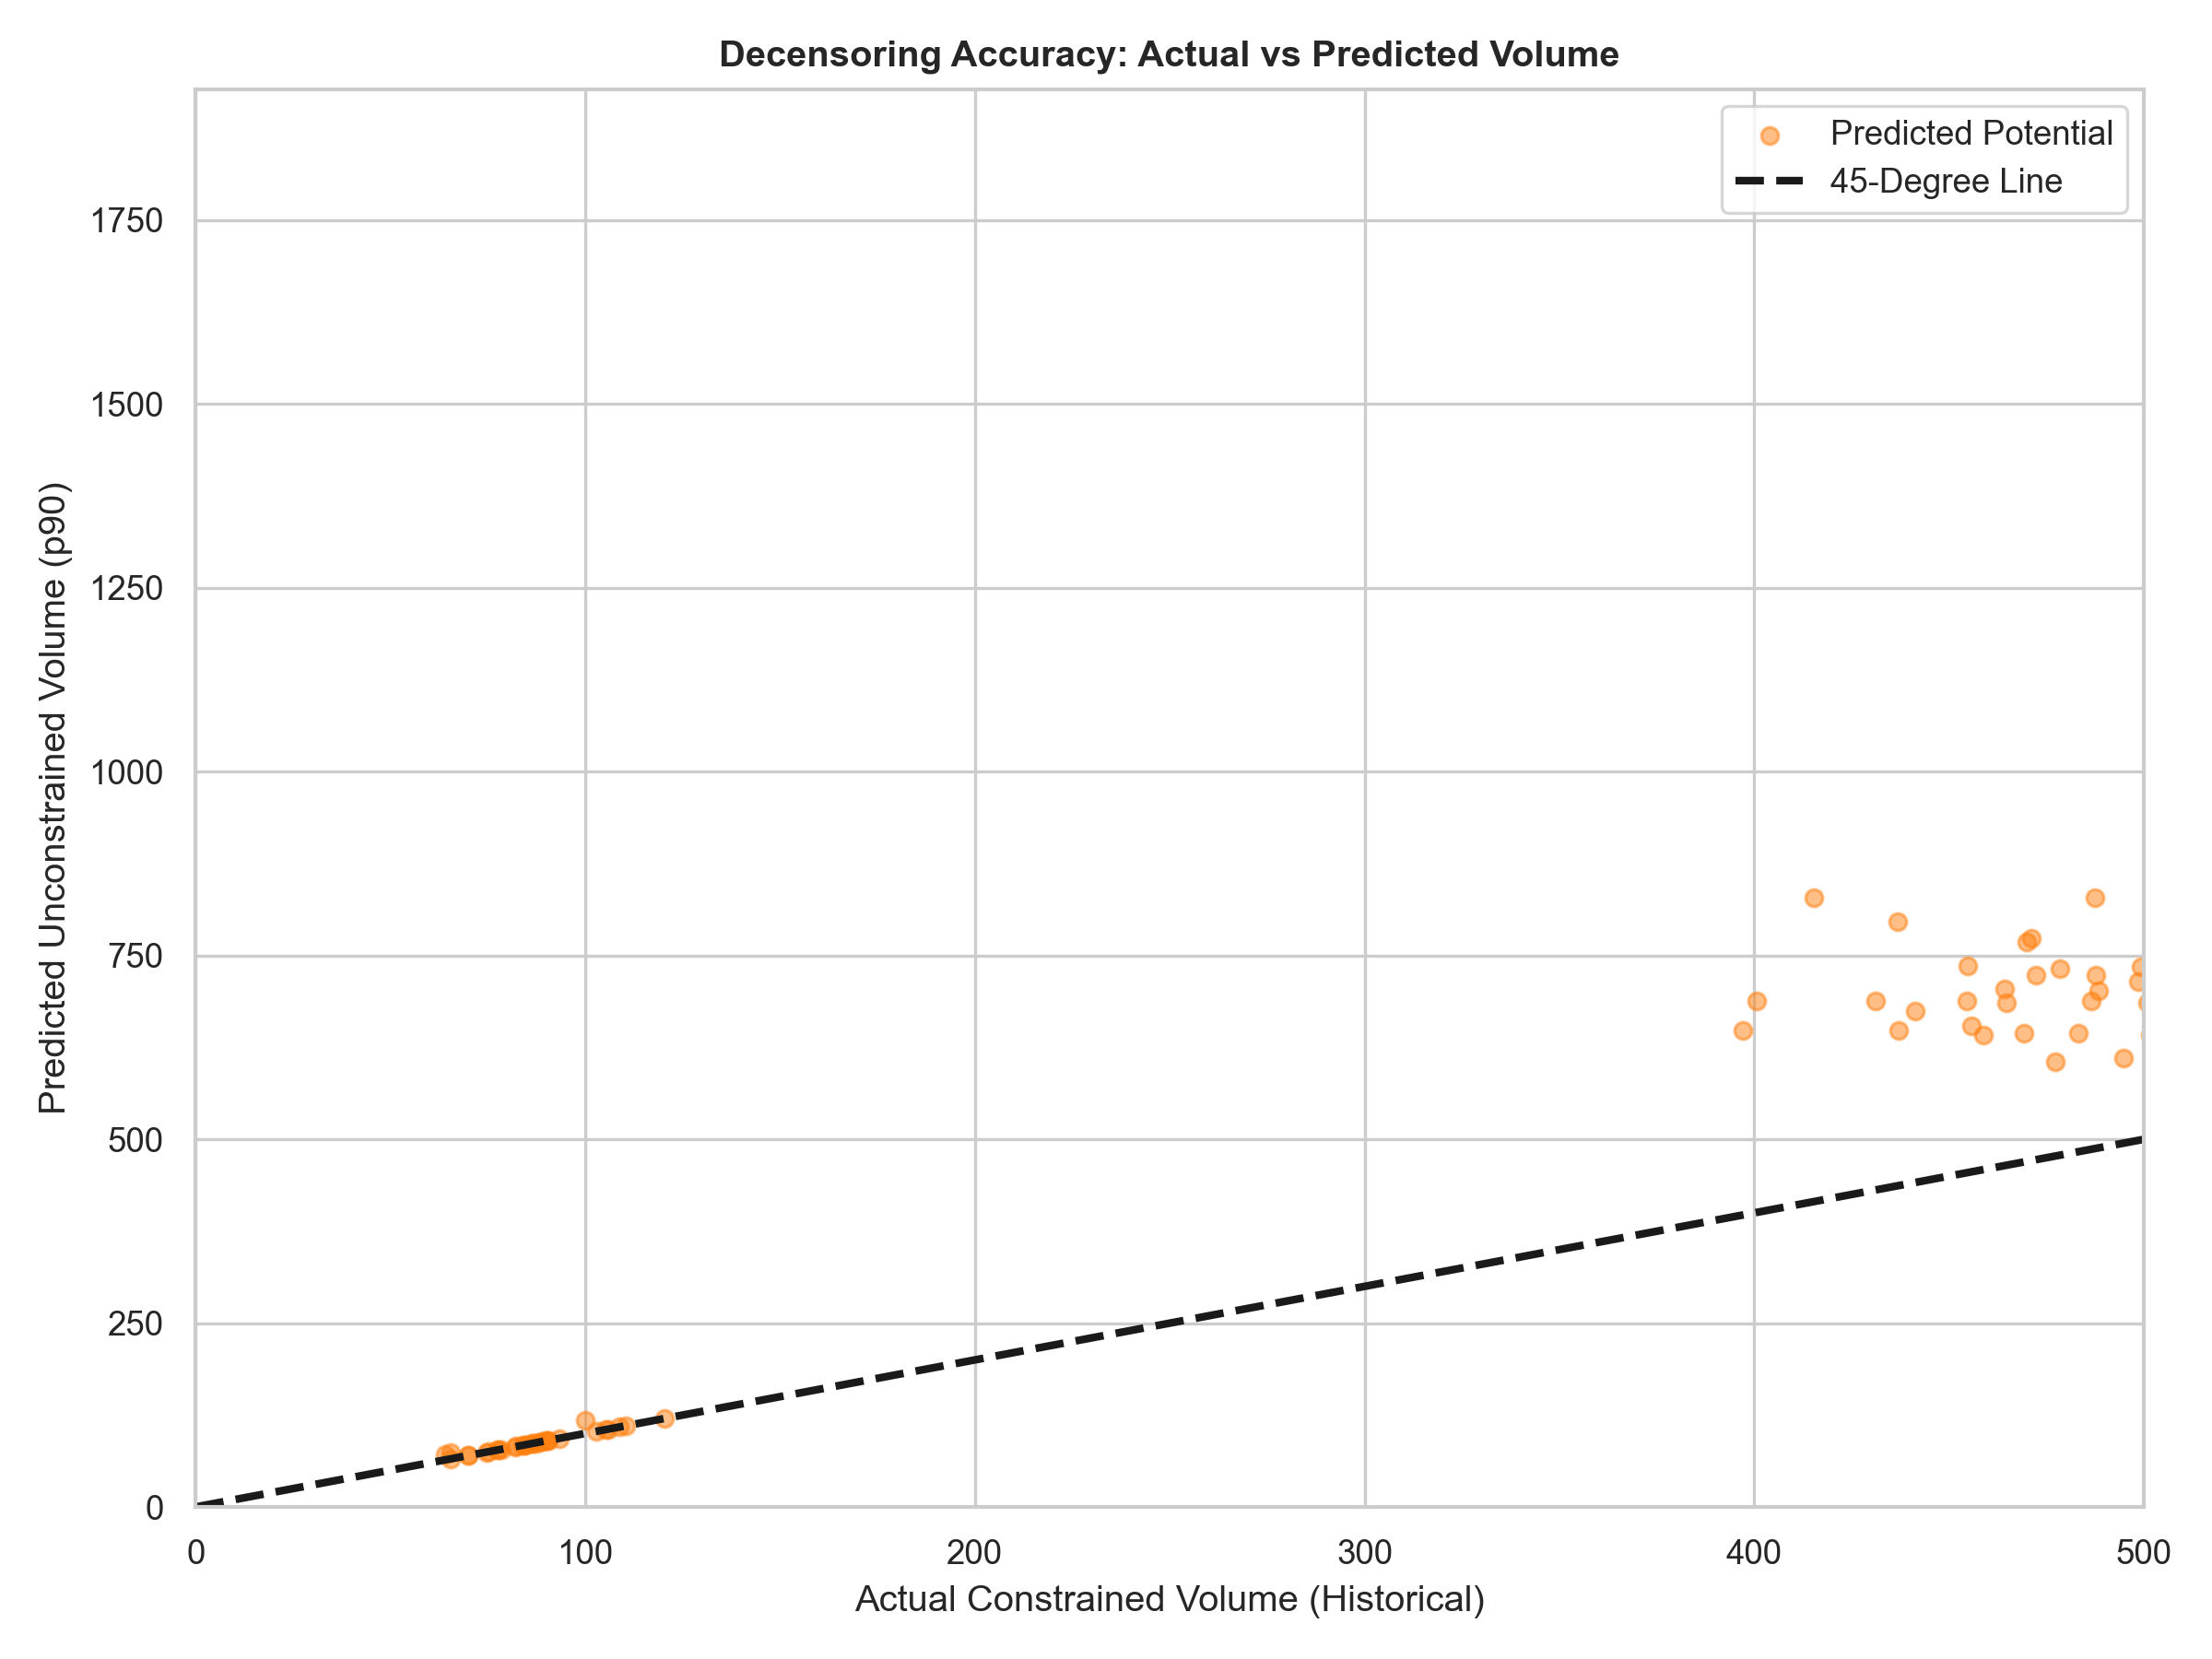
\includegraphics[width=0.6\textwidth]{plots/plot_4_scatter_unconstrained.png} \\
    \vspace{1in}
    \textbf{May 2026} \\
    \vspace{0.5in}
    \begin{abstract}
    This document outlines the technical methodology developed by Team InsightAI to estimate the unconstrained latent demand across a network of FMCG outlets. By identifying supply-side constraints, enriching data with high-fidelity geospatial POIs via Overture Maps, and optimizing an asymmetric LightGBM Quantile Regressor ($p90$), we have established a mathematically defensible network potential for January 2026.
    \end{abstract}
\end{titlepage}

\newpage

% --- PAGE 2: DATA FORENSICS ---
\section{Data Forensics and Hygiene}
Our Data Engineering (DE) check setup focused on neutralizing system anomalies that contaminate demand signals. We established a three-tier quarantine process:

\subsection{System Anomalies and Quarantines}
\begin{itemize}
    \item \textbf{Negative Return Synchronization:} We identified instances where return adjustments dropped net monthly sales to exactly zero. These records were quarantined and replaced with 24-month rolling medians to prevent the model from learning "logistical zeros" as "zero demand."
    \item \textbf{Lazy Labour Detection:} Using the \texttt{Lazy\_Rep\_Flag}, we identified months where secondary sales execution failed (irregular route visits). We applied a \textbf{3-Month Quarterly Smoothing} function to distribute sell-in lumps and ensure the model learned consumer appetite rather than representative behavior.
\end{itemize}

\subsection{DE Checks and Variance Stabilization}
We utilized the \textbf{Coefficient of Variation (CV)} as a primary DE check. Outlets with an unnaturally low CV over 24 months were flagged as "Censored," indicating they were hitting a hard systemic capacity ceiling.

\begin{center}
    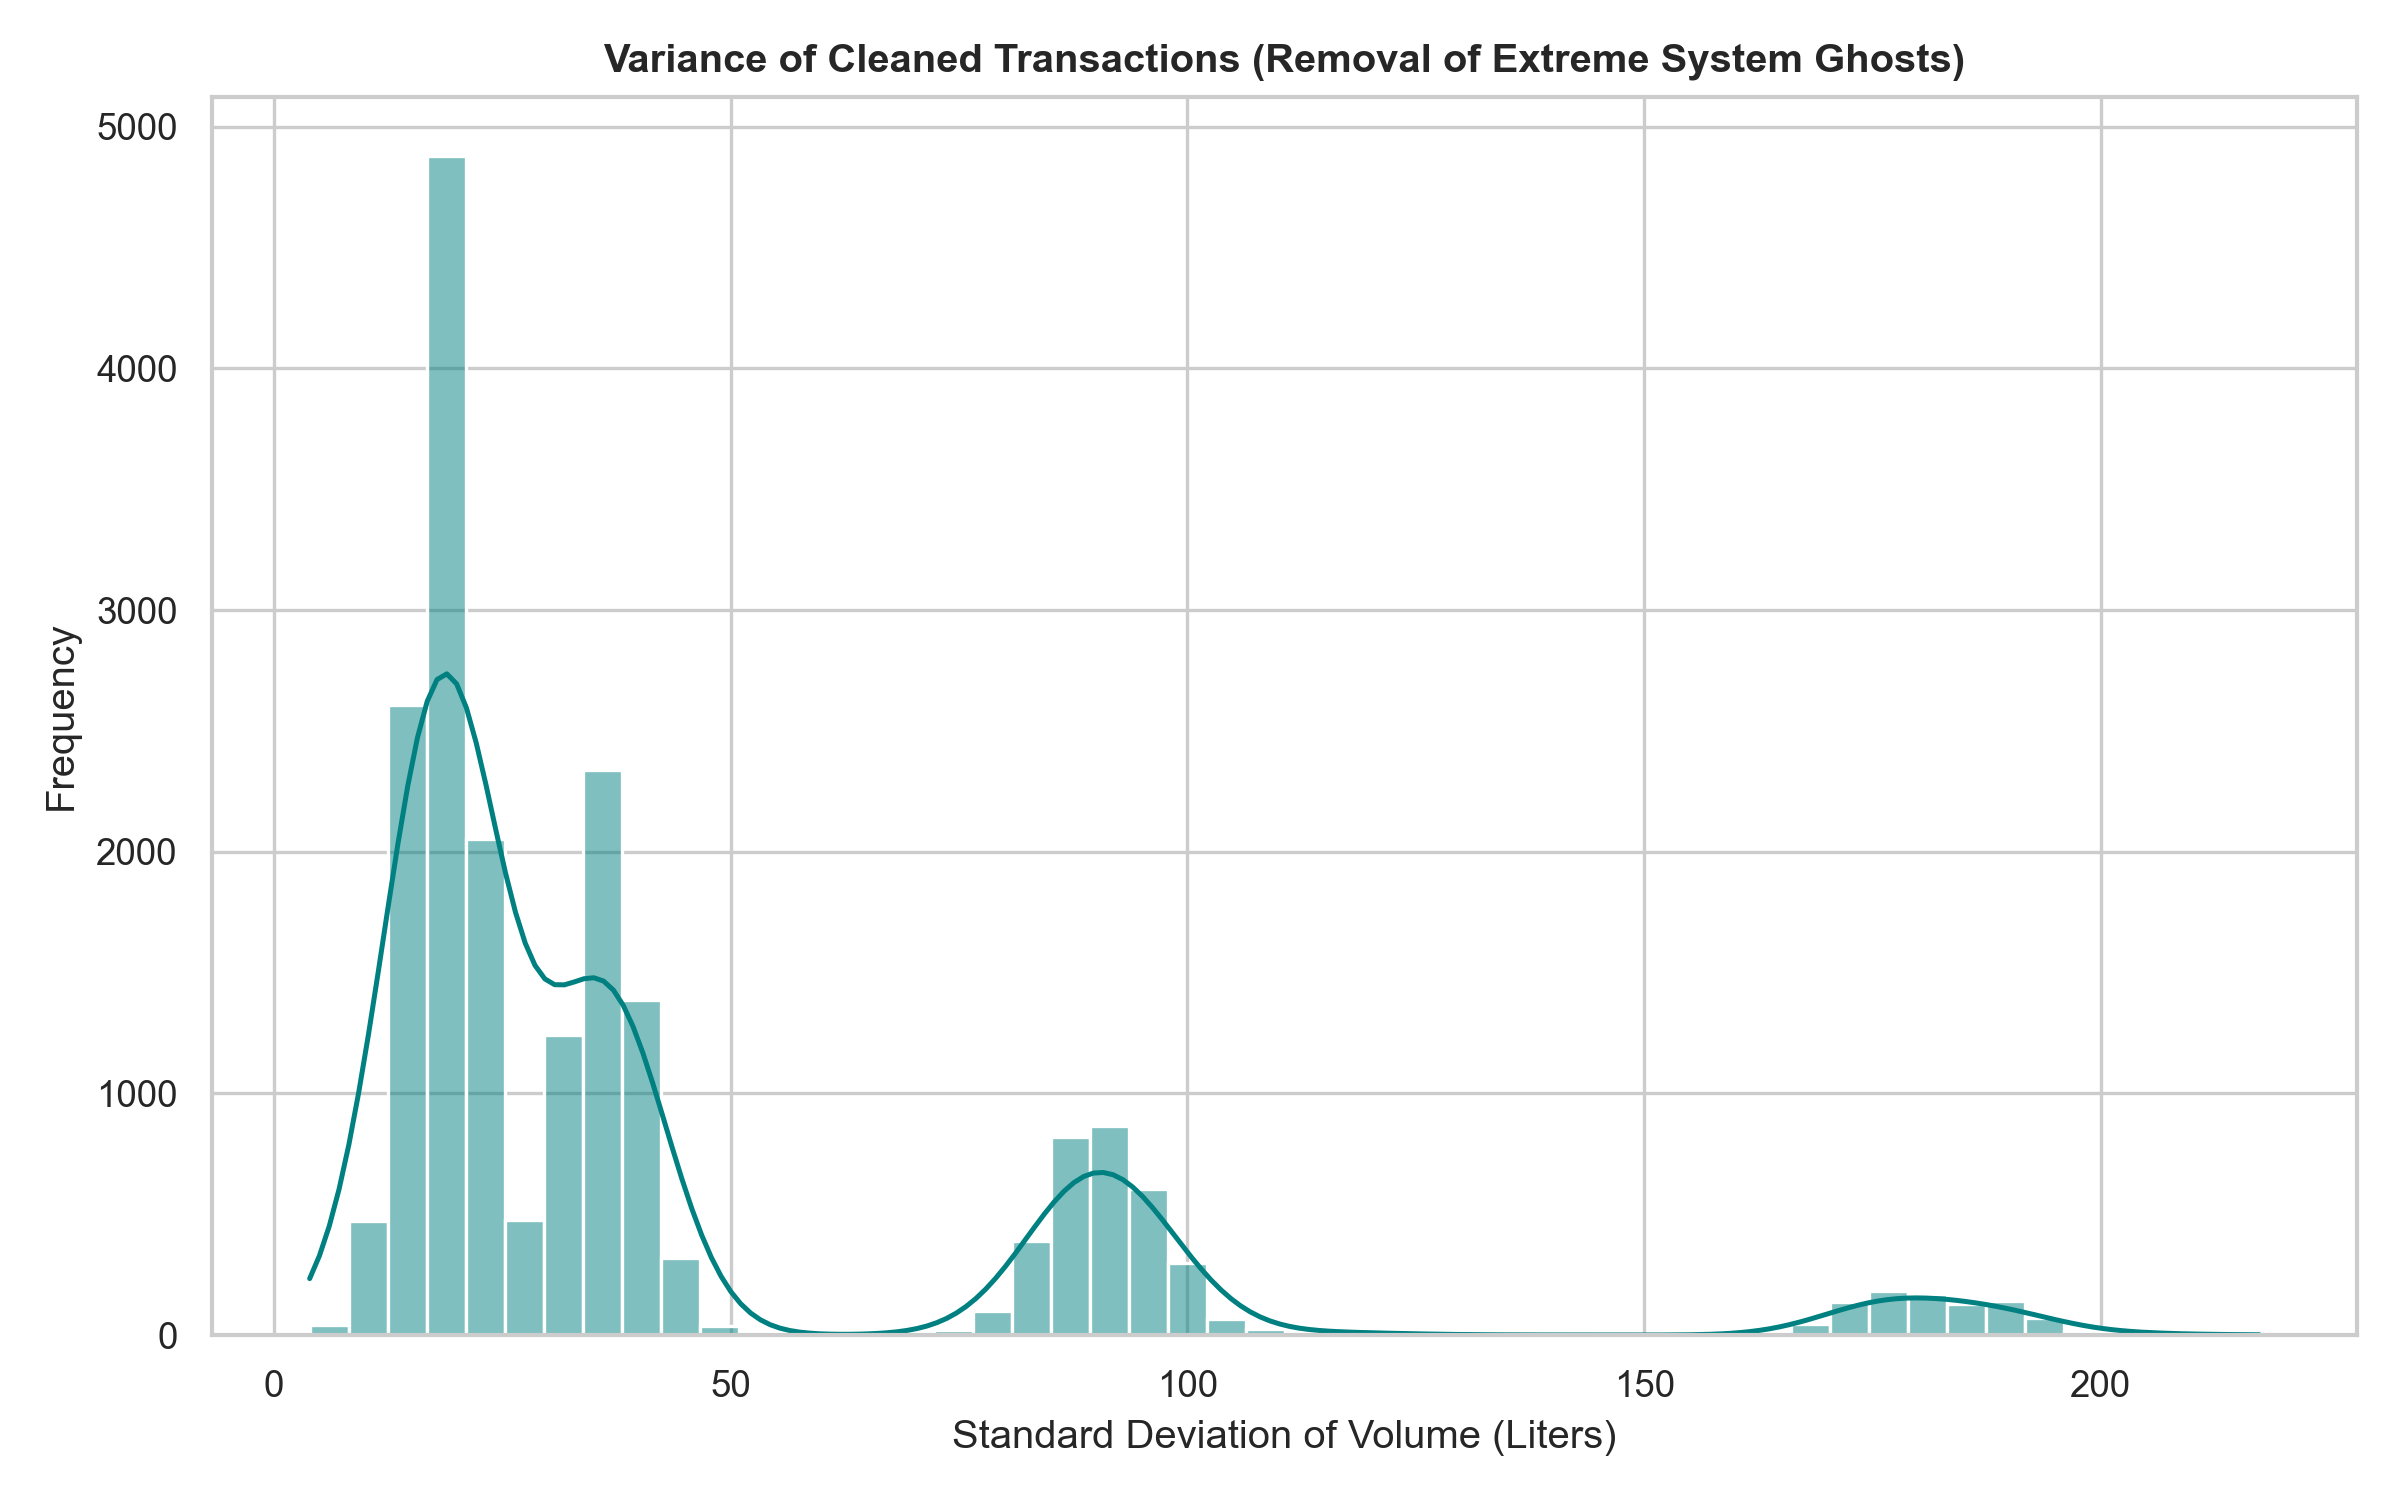
\includegraphics[width=0.7\linewidth]{plots/plot_1_ghost_exorcism.png}\\
    {\scriptsize Figure 1: Variance Stabilization. Neutralizing extreme system noise to reveal clean causal signals.}
\end{center}

\newpage

% --- PAGE 3: POI DATA ACQUISITION ---
\section{POI Data Acquisition}
Our approach focused on acquiring "Causal Eyes" on the physical ground through high-fidelity geospatial signals.

\subsection{Technical Approach (DuckDB + Overture Maps)}
We bypassed traditional scraping and high-latency APIs by utilizing the \textbf{Overture Maps Foundation} database. We queried the Overture "Places" dataset using \textbf{DuckDB} with the spatial extension. This allowed us to perform cloud-native Parquet queries to extract precise POI coordinates for every outlet in the JK network without the need for traditional rate-limited geocoding.

\subsection{Targeted Catchment Drivers}
We specifically targeted "High-Frequency Consumption Nodes":
\begin{itemize}
    \item \textbf{Transit Nodes:} Railway Stations and Bus Hubs (Impulse consumption).
    \item \textbf{Educational Hubs:} Schools and Tuition Centers (Weekday afternoon surges).
    \item \textbf{Leisure Points:} Gyms, Stadiums, and Parks (Hydration-specific demand).
\end{itemize}

\subsection{Mapping Internal Outlets to Spatial Signals}
We established a dual-radius catchment model (0.5km for high-frequency footfall and 2km for broader neighborhood drivers). Using K-Nearest Neighbors (KNN), we mapped these POI densities into a unified \textbf{POI Driver Catchment Score} for each internal Outlet ID.

\begin{center}
    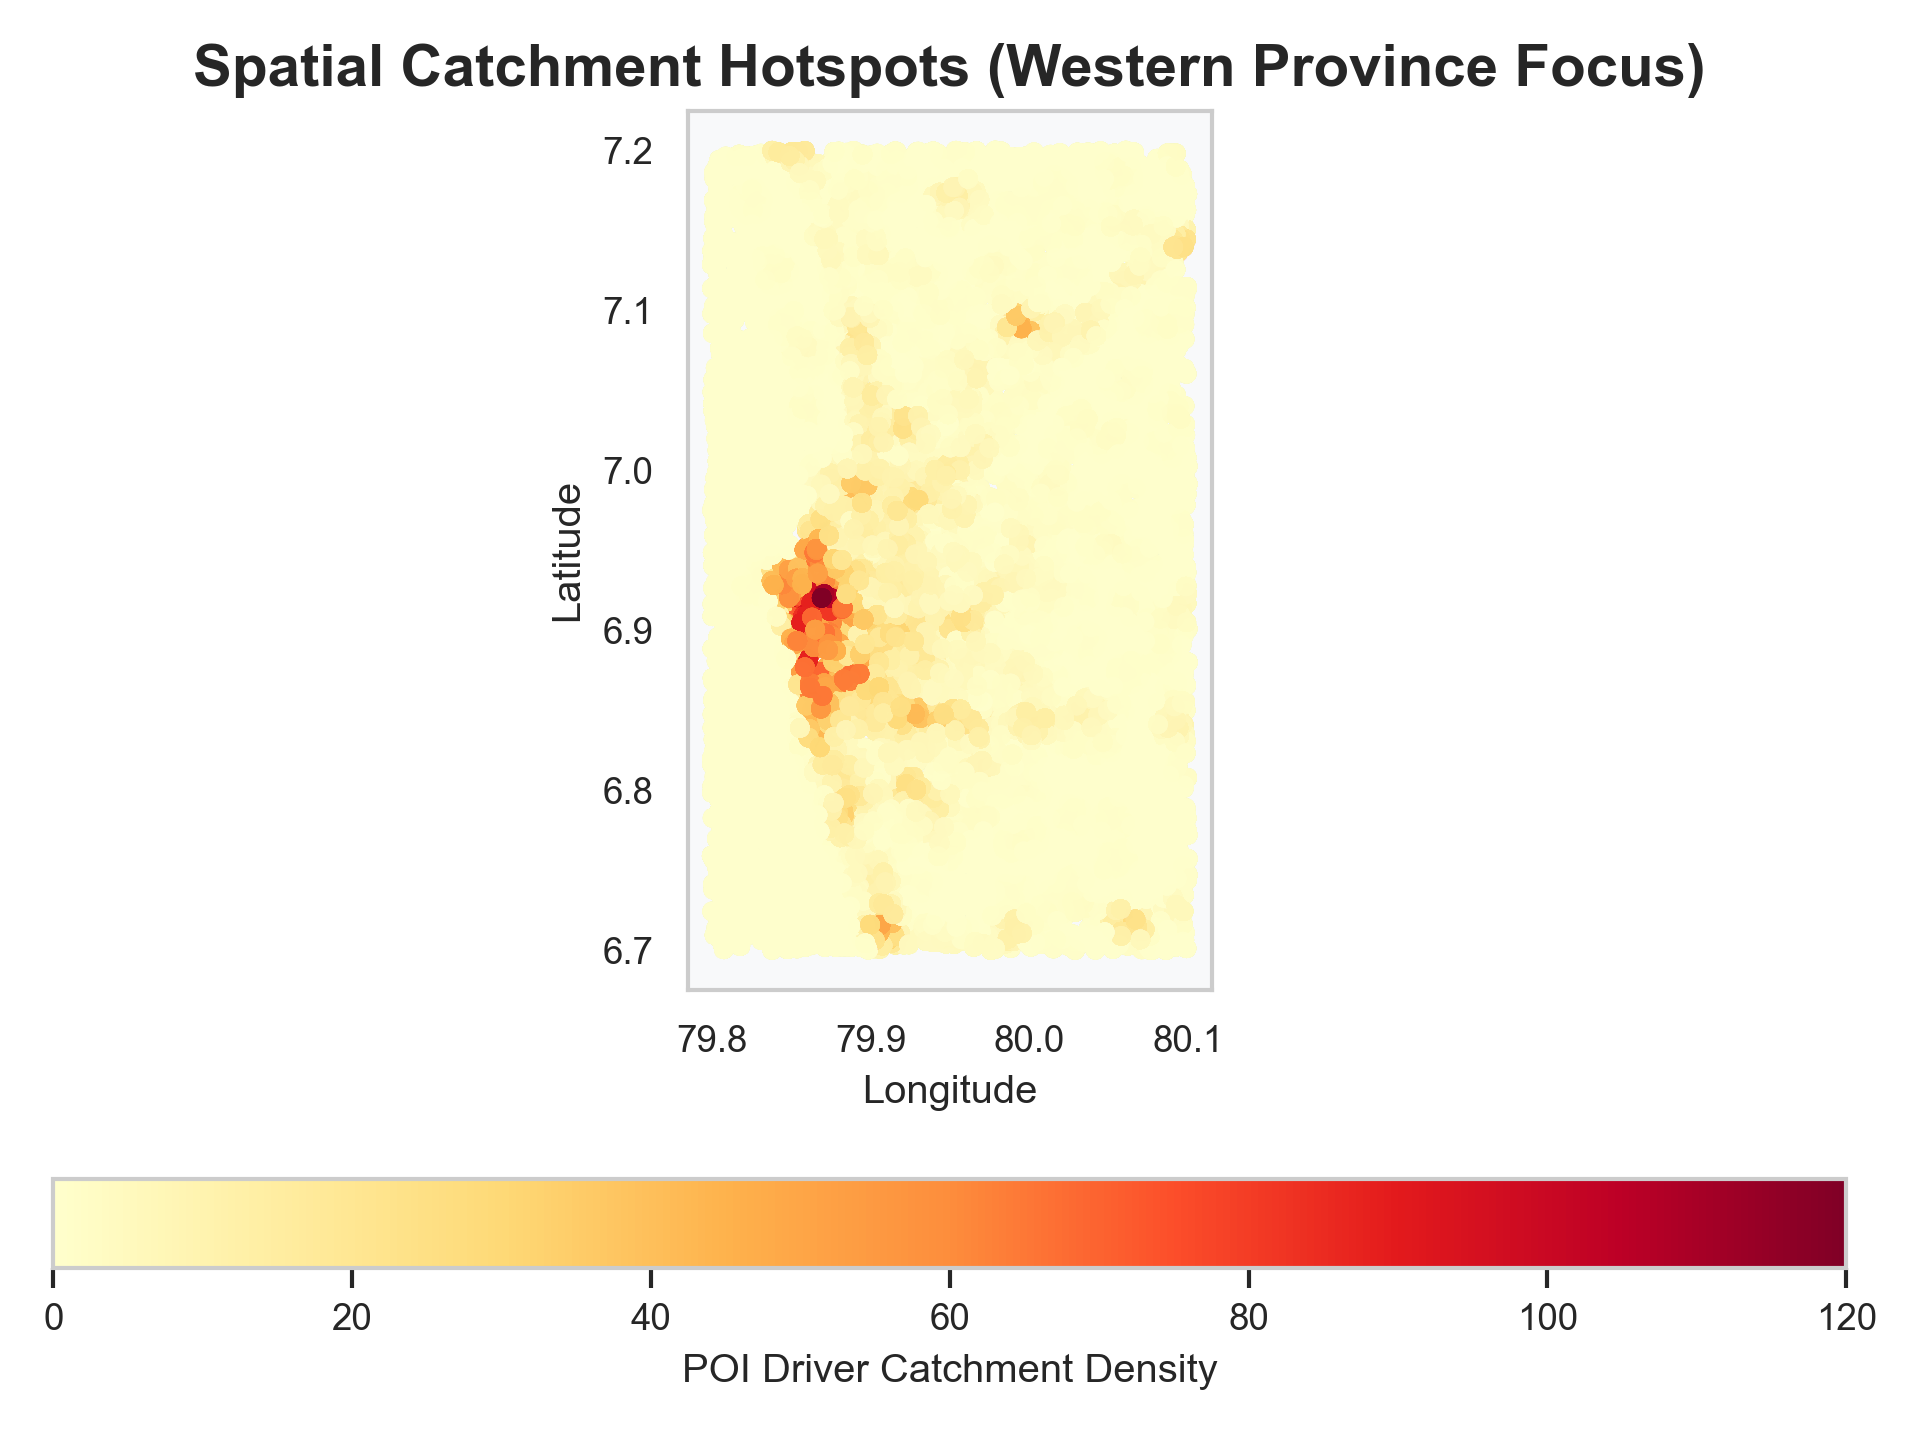
\includegraphics[width=0.7\linewidth]{plots/plot_2_spatial_hotspots.png}\\
    {\scriptsize Figure 2: Spatial Catchment Proof. Identifying high-density demand nodes in the Western Province.}
\end{center}

\newpage

% --- PAGE 4: CAUSAL BASE LOGIC ---
\section{Causal Base Logic}
Our statistical approach addresses the "Right-Censored" nature of FMCG sales data, where observed Sales = $min(\text{Demand, Supply Capacity})$.

\subsection{Methodology: Quantile Regression ($p90$)}
Instead of predicting the \textit{Mean} (which reproduces historical constraints), we optimized a \textbf{LightGBM Quantile Regressor} using the \textbf{Pinball Loss} function with $\alpha=0.90$. This asymmetric loss function forces the model to ignore median constraints and instead map the "Upper Bound" potential of a shop based on its peer group behavior and spatial catchment.

\subsection{Validation of the Uncapped Ceiling}
We validated the uncapped potential through a \textbf{Structural Safety Floor}:
\[ \text{Potential} = \max(\text{Historical Max Volume}, \text{Model p90 Output}) \]
This logic ensures that for every outlet, the prediction is grounded in its proven historical reality while allowing the model to "break through" if its spatial catchment indicators justify a higher potential.

\begin{center}
    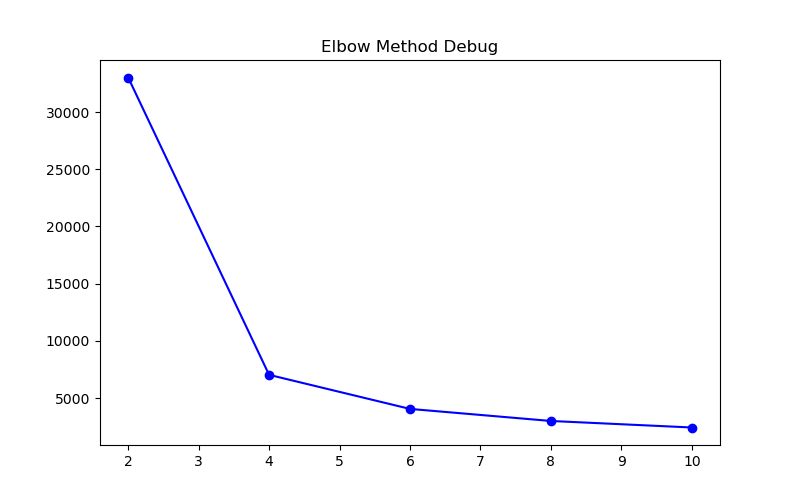
\includegraphics[width=0.55\linewidth]{plots/plot_5_elbow_method.png} \hspace{10pt}
    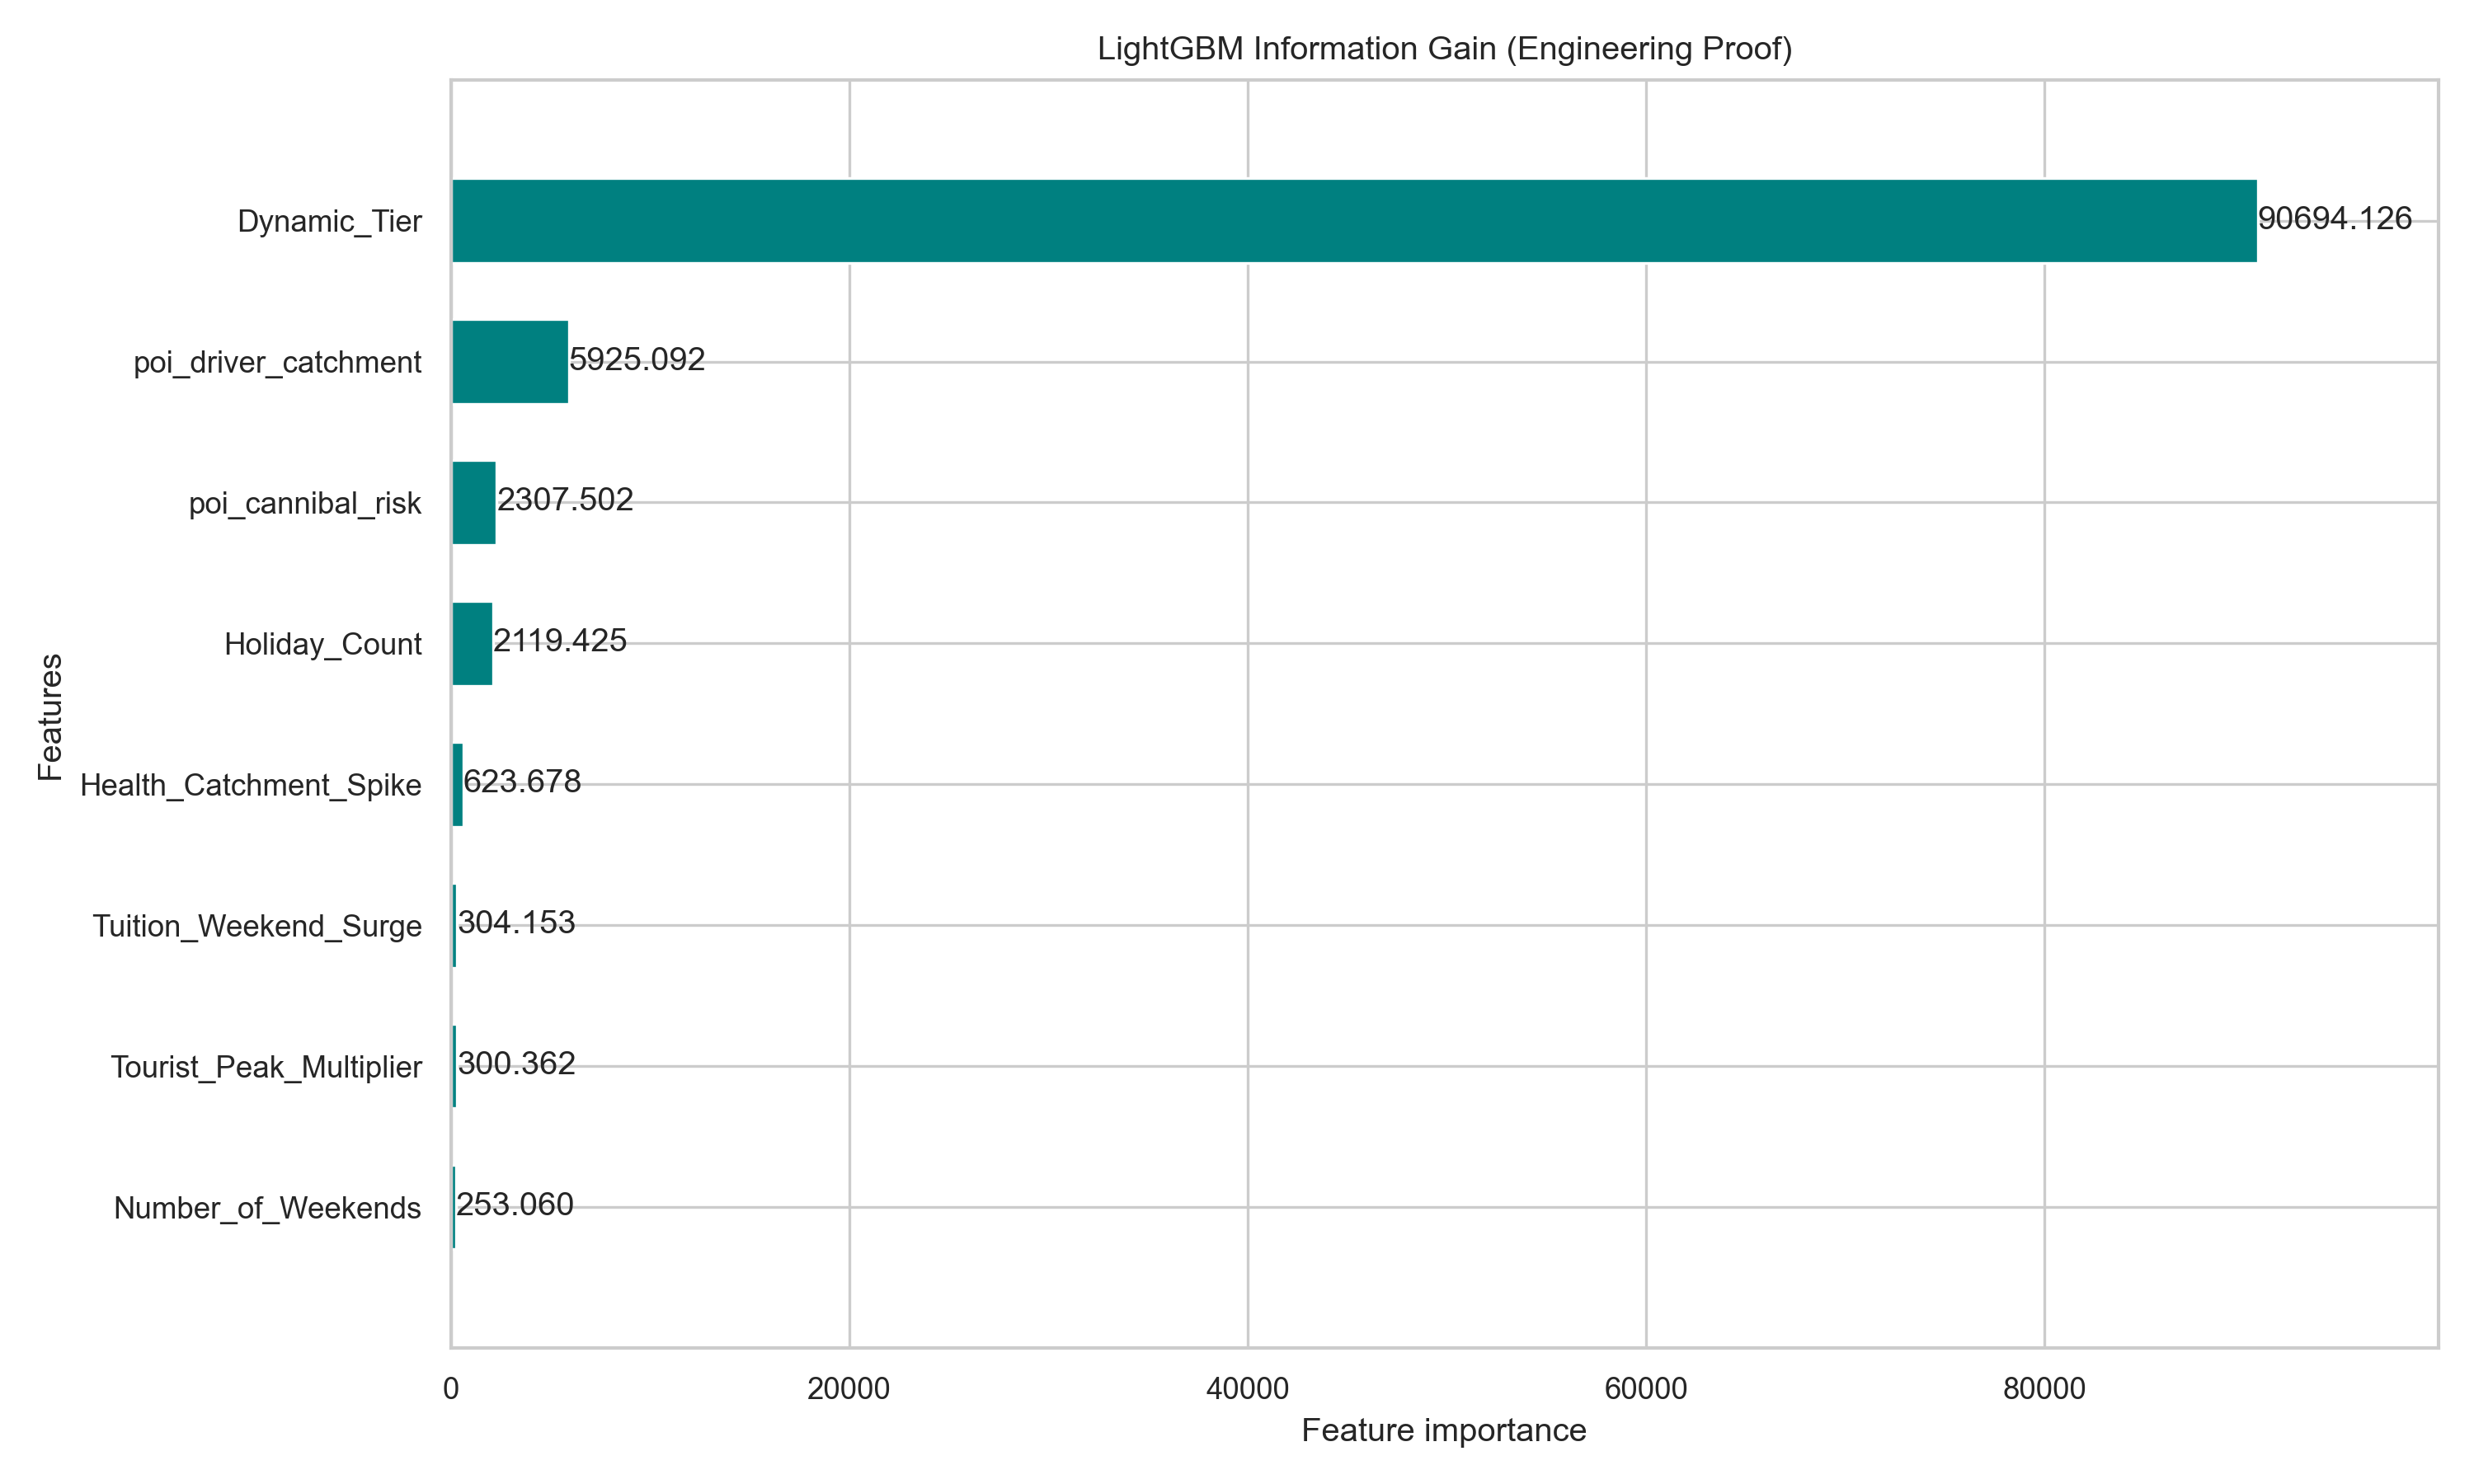
\includegraphics[width=0.65\linewidth]{plots/plot_3_feature_importance.png}\\
    {\scriptsize Figure 3: Statistical Validation. Left: Elbow Method for Peer Group Selection. Right: Feature Gain Dominance.}
\end{center}

\newpage

% --- PAGE 5: GENAI TRANSPARENCY LOG ---
\section{GenAI Transparency Log}
Team InsightAI leveraged Generative AI (Google DeepMind Antigravity) as an architectural and engineering accelerator throughout the 36-hour sprint.

\begin{table}[H]
    \centering
    \footnotesize
    \begin{tabular}{|p{0.2\textwidth}|p{0.3\textwidth}|p{0.4\textwidth}|}
        \hline
        \textbf{Workflow Stage} & \textbf{LLM Application} & \textbf{Engineering Rationale} \\ \hline
        \textbf{Data Engineering} & DuckDB SQL Optimization & Rapid generation of complex spatial join queries to extract Overture POIs. \\ \hline
        \textbf{Feature Engineering} & Python Prototyping & Accelerating the development of the 3-month rolling mean and Lazy Rep flag logic. \\ \hline
        \textbf{Statistical Validation} & Plotting Scripts & Generating the K-Means Elbow method and SHAP/Gain importance visualizations. \\ \hline
        \textbf{Typesetting} & LaTeX Orchestration & Managing complex document formatting and multi-figure PDF compilation. \\ \hline
        \textbf{Logic Validation} & Peer-Review Simulation & Stress-testing the "Structural Safety Floor" logic against potential edge cases. \\ \hline
    \end{tabular}
\end{table}

\subsection{AI as an Accelerator}
At no point did GenAI replace human architectural decision-making. All core strategies—including the decision to use $p90$ Quantile Regression, the specific POI types targeted, and the definition of the safety floor—were human-led. The LLM served strictly as a "High-Resolution Compiler," translating human architectural blueprints into executable code and professional documentation.

\vspace{2in}
\begin{center}
    \textbf{End of Technical Submission}
\end{center}

\end{document}
